\chapter{Proses Bisnis dan Pengumpulan Data Fisik}

\section{Proses Bisnis}
Melampirkan KK lama yang akan dipecah Untuk istri yang bercerai dengan mantan suaminya tetapi belum memiliki  surat cerai. Salah satu solusi cara mengurus KK setelah cerai yaitu dengan mengembalikan data istri ke KK milik orang tua atau Istri membuat KK sendiri dengan Istri sebagai kepala keluarga di KK tersebut. 
Cara mengurus KK setelah bercerai yaitu kamu perlu mendatangi kantor kelurahan setempat untuk mengisi formulir permohonan Kartu Keluarga baru dengan membawa berkas persyaratan yang dibutuhkan. Setelah itu kamu mendatangi kantor kecamatan untuk proses lebih lanjut untuk proses penerbitan KK atau Kartu Keluarga yang baru.
Dalam pembuatan KK seorang janda tidak diwajibkan untuk meminta tanda tangan mantan suami. Apabila pihak kecamatan tidak mengeluarkan kartu keluarga maka dapat diajukan keberatan atau komplain ke instansi yang lebih tinggi yaitu ke walikota. Permohonan pembuatan KK dapat diajukan secara tertulis dan meminta jawaban secara tertulis juga dari kecamatan. Apabila tidak ada tanggapan maka dapat jawaban tertulis dari kecamatan itulah yang bisa dijadikan bukti untuk dilaporkan kepada Ombudsman berkaitan dengan pelayanan publik pembuatan kartu keluarga.

Cara mengurus KK setelah bercerai kamu memerlukan persyaratan berikut ini :
\begin{enumerate}
	\item Mengisi persyaratan berupa formulir permohonan Kartu Keluarga atau KK;.
	\item Menyerahkan fotocopy akta kelahiran dari desa atau kelurahan setempat;.
	\item Bagi istri yang sudah bercerai hanya perlu menyerahkan fotocopy surat cerai;.
\end{enumerate}
	\begin{figure}[H]
		\centering
		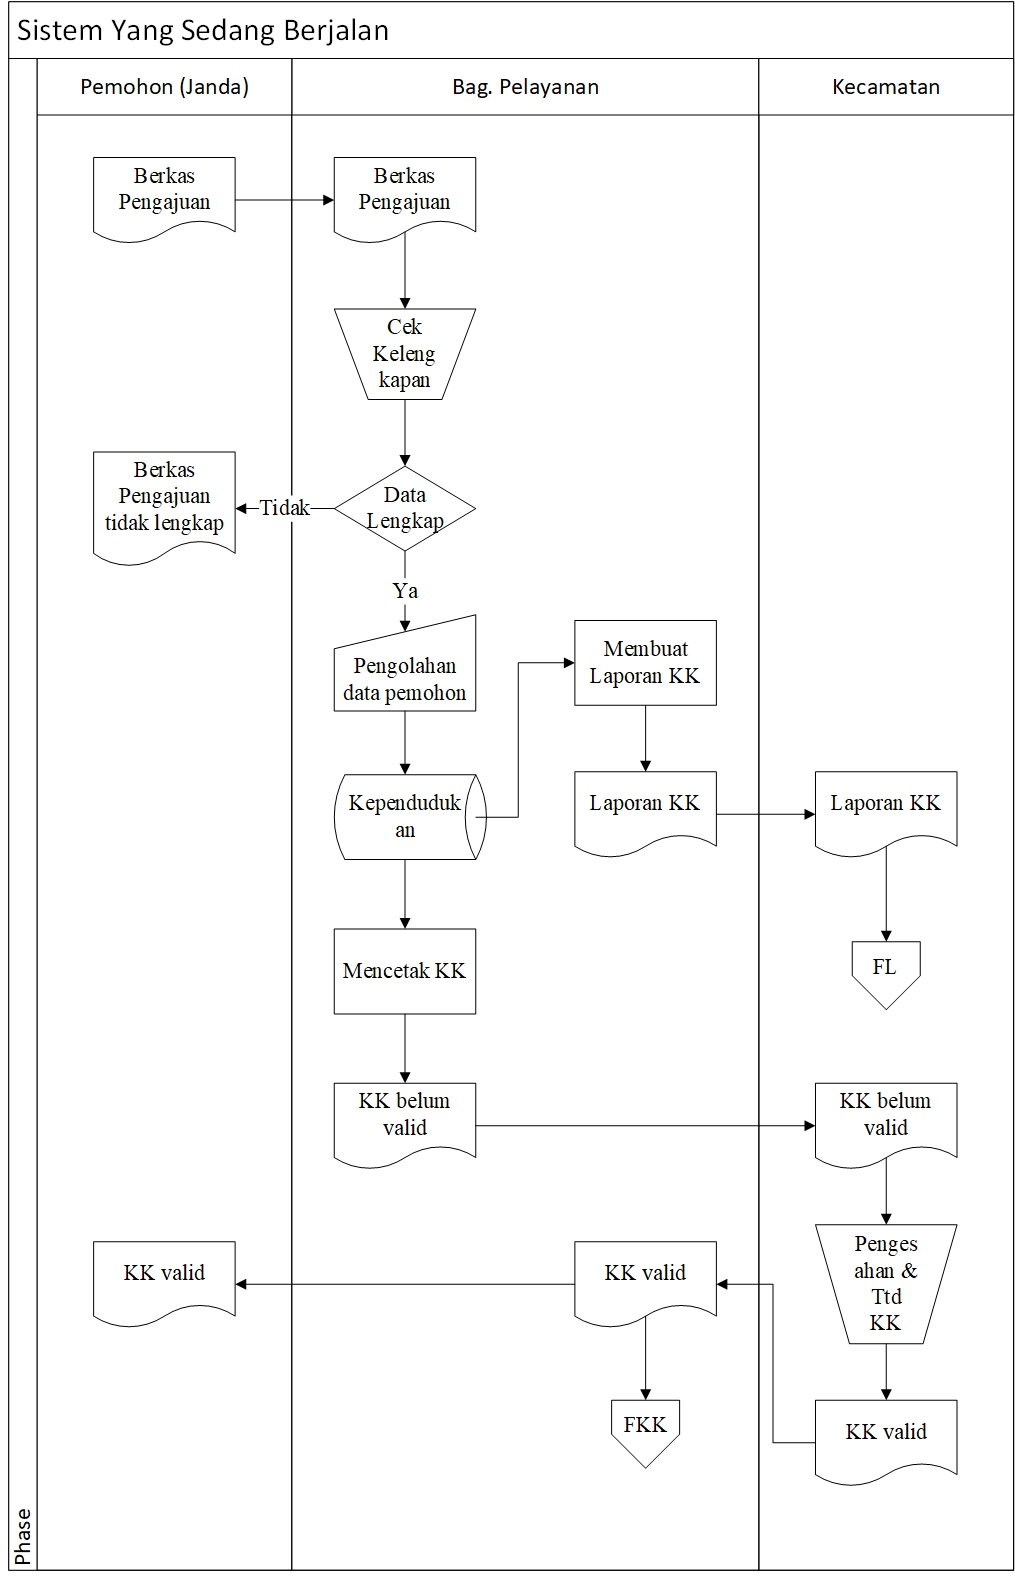
\includegraphics[width=10cm]{figures/flowmap.jpg}
		\caption{Flowmap Sistem Yang Sedang Berjalan.}
	\end{figure}
Keterangan:
\begin{enumerate}
	\item Berkas pengajuan meliputi formulir isian kartu keluarga, foto copy akta kelahiran, dan foto kopi akta cerai;.
	\item FL = Berkas Laporan;.
	\item FKK = Berkas KK;.
\end{enumerate}
\section{Data Fisik}
Berkas fisik yang akan digunakan dalam perancangan databse, yaitu sebagai berikut:
\begin{enumerate}

	\item Kartu Keluarga Keluarga Pertama
	\begin{figure}[H]
		\centering
		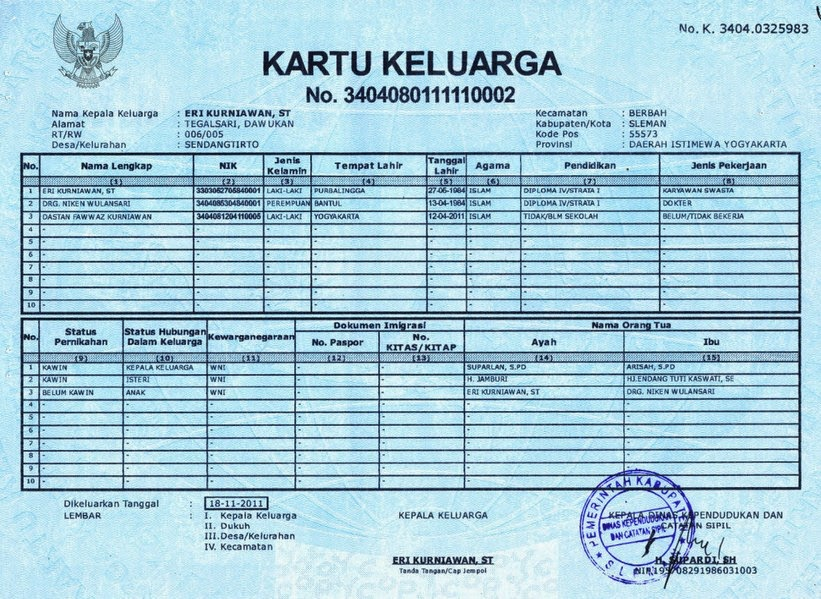
\includegraphics[width=12cm]{figures/kk.jpg}
		\caption{Kartu Keluarga.}	
	\end{figure}

	\item Akta Kelahiran
	\begin{figure}[H]
		\centering
		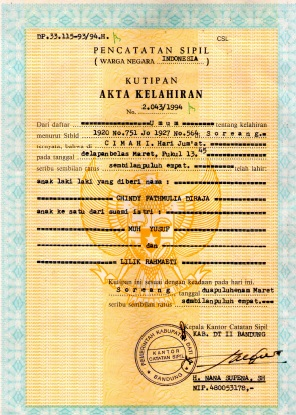
\includegraphics[width=10cm]{figures/akte.jpg}
		\caption{Akta Kelahiran.}	
	\end{figure}

	\item Formulir F-1.21
	\begin{figure}[H]
		\centering
		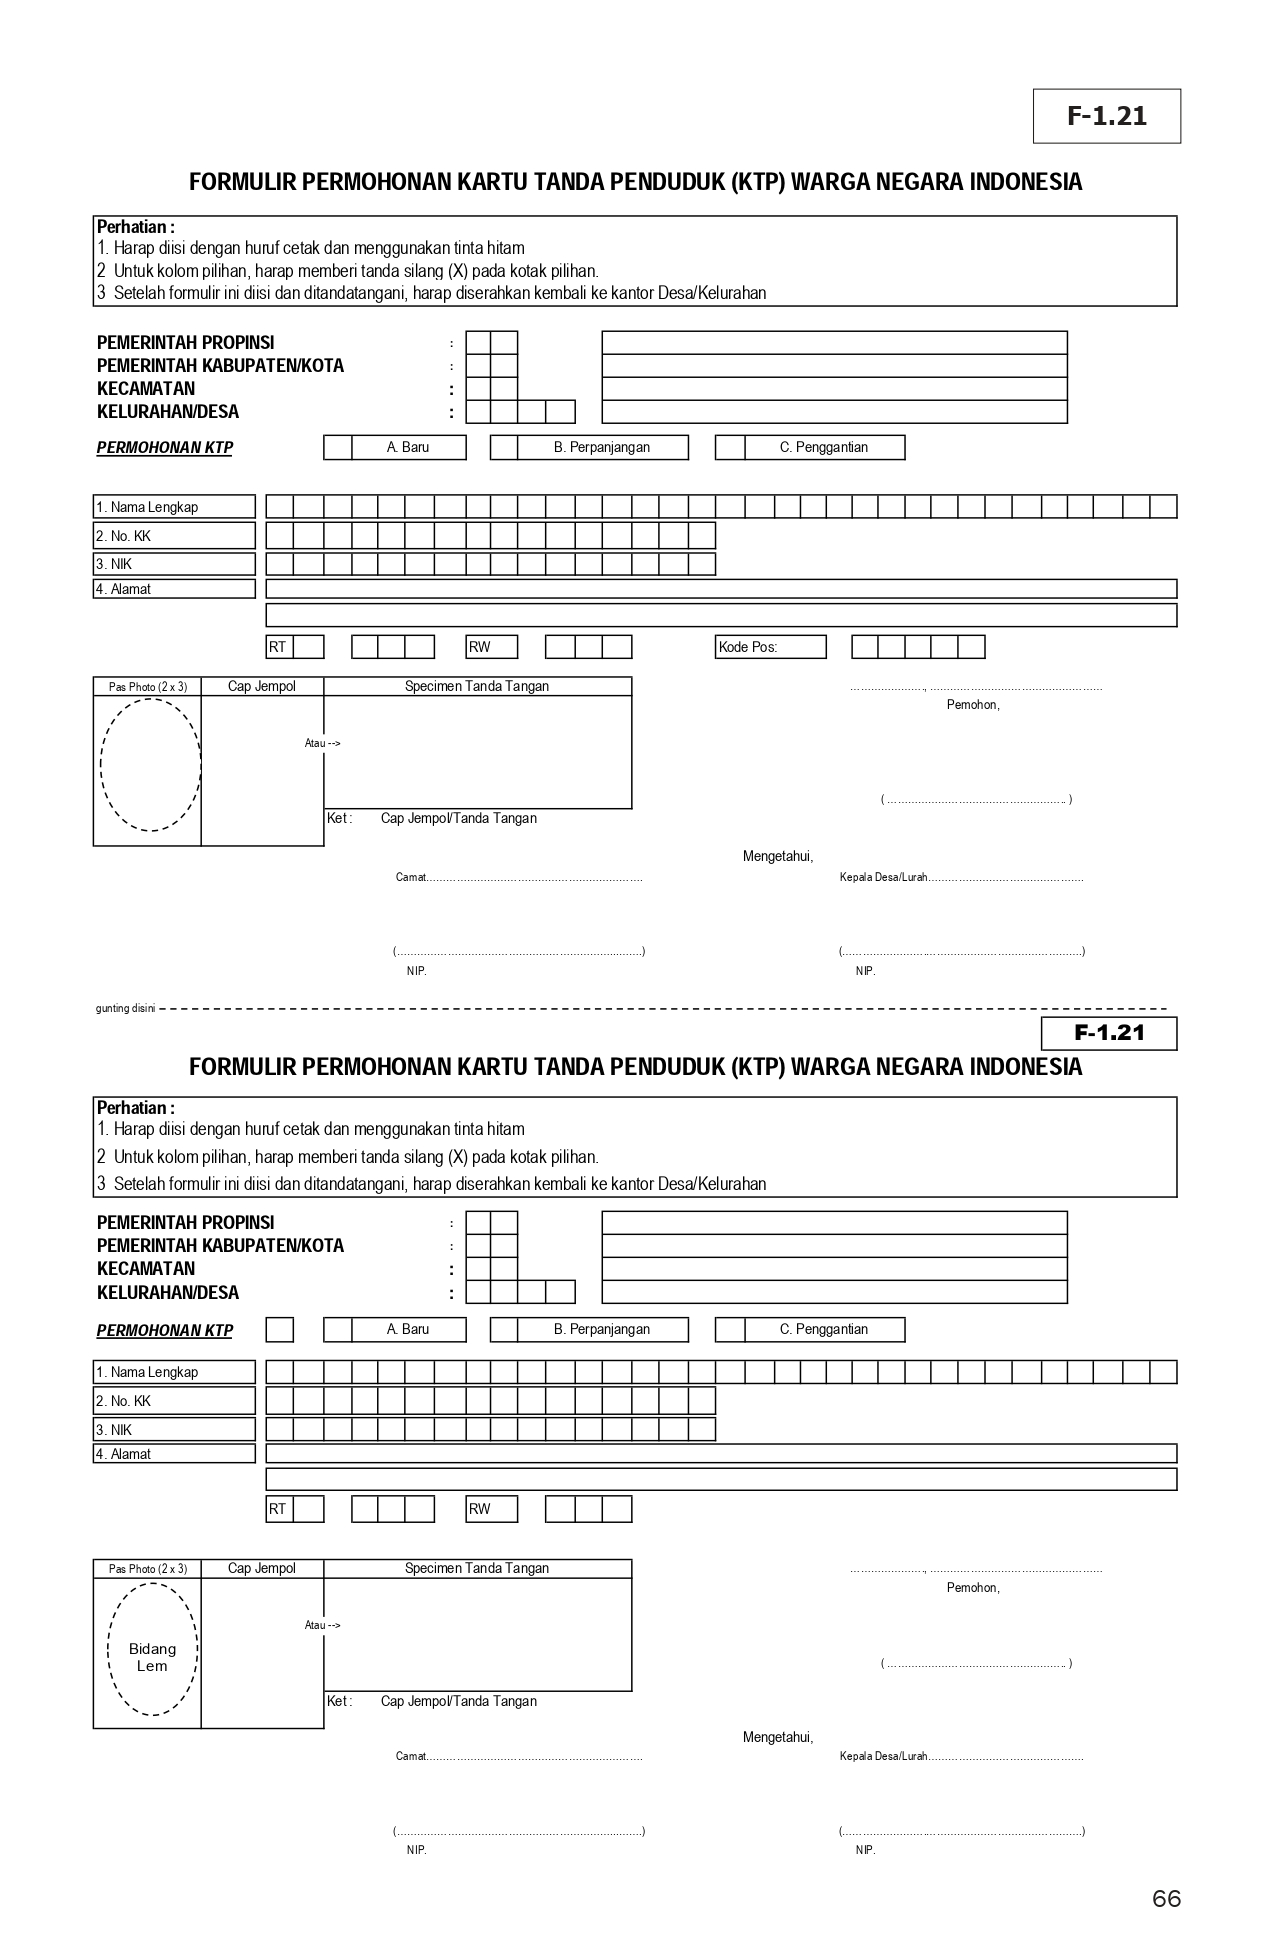
\includegraphics[width=10cm]{figures/formulir.jpg}
		\caption{Formulir F-1.21.}	
	\end{figure}

	\item Akta Cerai
	\begin{figure}[H]
		\centering
		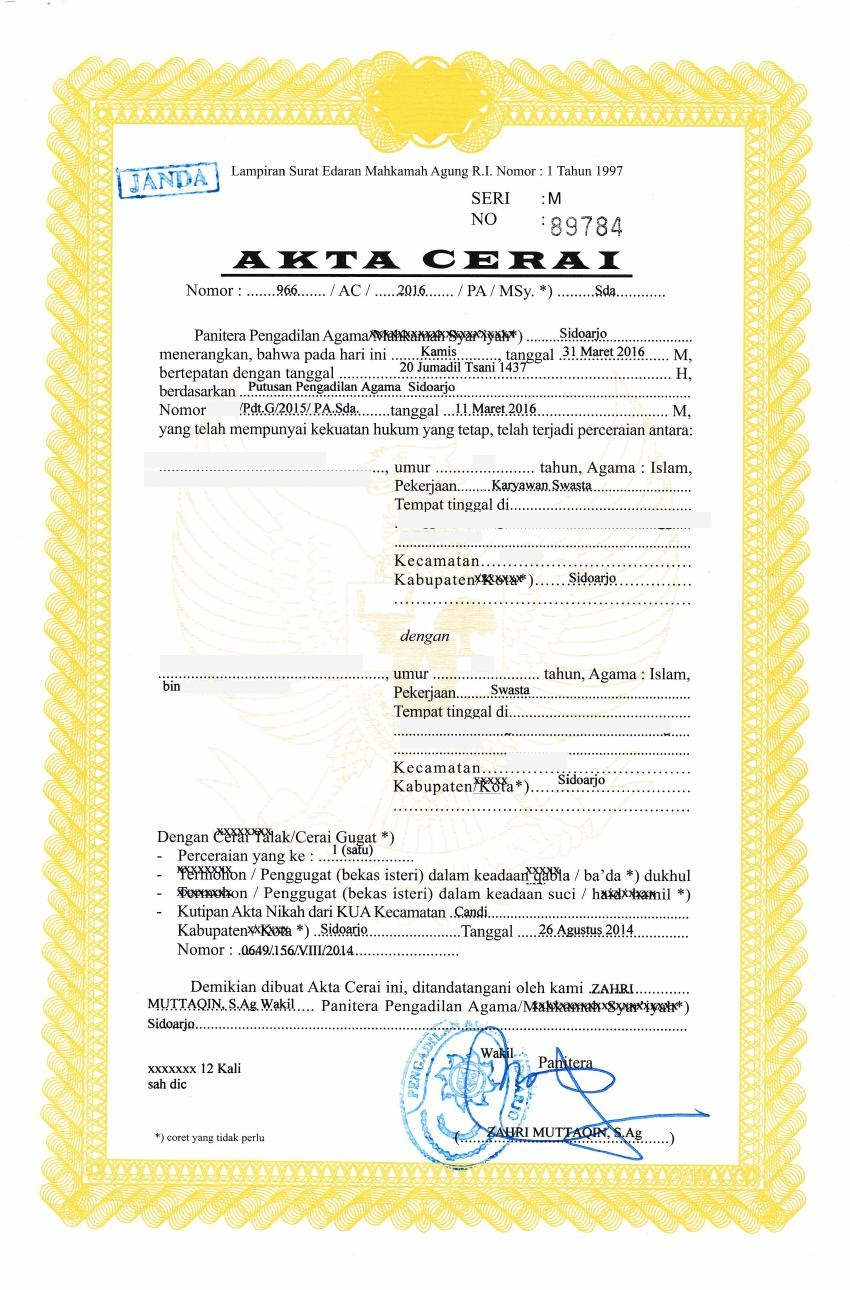
\includegraphics[width=10cm]{figures/aktacerai.jpg}
		\caption{Akta Cerai}	
	\end{figure}
\end{enumerate}